%% Quiz 4 on page 22/23

\documentclass{hw}

\usepackage{multicol}

\usepackage{tikz}
\usetikzlibrary{automata,positioning}

\begin{document}

\begin{enumerate}
\item Two competing companies, Pollution Products and Environmental Hazards, simultaneously introduce
new enzyme laundry detergents. Market tests indicate that during a year, Pollution keeps 60\% of
its customers and loses 40\% of its customers to Environmental. On the other hand, Environmental
keeps half of its customers and loses the other half to Pollution. Set up this process as a Markov
chain. Determine the transition matrix and sketch a state diagram.

\begin{minipage}{0.5\textwidth}
\[
\begin{array}{c | c c}
& \text{Pollution} & \text{Environmental}\\
\hline
\text{Pollution} & .6 & .4\\
\text{Environmental} & .5 & .5
\end{array}
\]
\end{minipage}
\begin{minipage}{0.5\textwidth}
\begin{center}
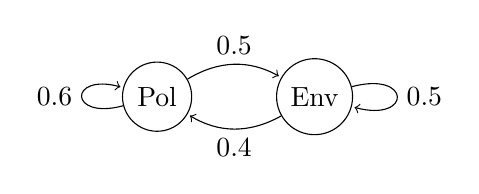
\begin{tikzpicture}[shorten >=1pt,node distance=2cm,on grid,auto]
   \node[state] (q_0) {Pol};
   \node[state] (q_1) [right=of q_0] {Env};
   % \node[state] (q_2) [below right=of q_0] {$q_2$};
   % \node[state,accepting](q_3) [below right=of q_1] {$q_3$};
    \path[->]
    (q_0) edge [bend left] node {0.5} (q_1)
          edge [loop left] node {0.6} ()
    (q_1) edge [bend left] node {0.4} (q_0)
          edge [loop right] node {0.5} ();
\end{tikzpicture}
\end{center}
\end{minipage}

\item Abigail spends her entire weekly allowance on either candy or toys. If she buys candy 1 week,
she is 60\% sure to buy toys the next week. The probability that she buys toys in two successive
weeks is 1/5. Set up this process as a Markov chain. Determine the transition matrix and sketch a
state diagram.

\begin{minipage}{0.5\textwidth}
\[
\begin{array}{c | c c}
& \text{Candy} & \text{Toys}\\
\hline
\text{Candy} & .4 & .6\\
\text{Toys} & .8 & .2
\end{array}
\]
\end{minipage}
\begin{minipage}{0.5\textwidth}
\begin{center}
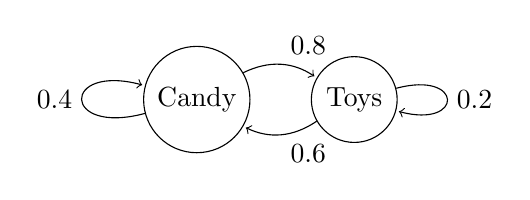
\begin{tikzpicture}[shorten >=1pt,node distance=2cm,on grid,auto]
   \node[state] (q_0) {Candy};
   \node[state] (q_1) [right=of q_0] {Toys};
   % \node[state] (q_2) [below right=of q_0] {$q_2$};
   % \node[state,accepting](q_3) [below right=of q_1] {$q_3$};
    \path[->]
    (q_0) edge [bend left] node {0.8} (q_1)
          edge [loop left] node {0.4} ()
    (q_1) edge [bend left] node {0.6} (q_0)
          edge [loop right] node {0.2} ();
\end{tikzpicture}
\end{center}
\end{minipage}

\item A political scientist in Canada discovered that of the children of Conservatives, 80\% vote
Conservative and the rest vote Labor; of the sons and daughters of Labor supporters, 60\% vote
Labor, 20\% vote Conservative, and 20\% vote for the New Democratic Party (NDP); and of the
offspring of NDP followers, 75\% vote NDP, 15\% vote Labor, and 10\% vote Conservative.
\begin{enumerate}
\item What is the probability that the grandchild of a Conservative will vote for the NDP?
\begin{quote}
The probability that a grandchild of a conservative will vote for the NDP is $(.2)(.2)$
\end{quote}
\item Set up this process as a Markov chain, with steps corresponding to successive generations.
Determine the transition matrix and sketch the state diagram.

\begin{minipage}{0.5\textwidth}
\[
\begin{array}{c | c c c}
& \text{L} & \text{C} & \text{N}\\
\hline
\text{L} & .6 & .2 & .2\\
\text{C} & .2 & .8 & 0\\
\text{N} & .15 & .1 & .75
\end{array}
\]
\end{minipage}
\begin{minipage}{0.5\textwidth}
\begin{center}
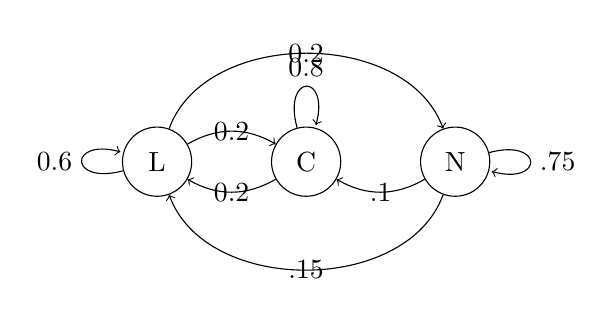
\begin{tikzpicture}%[shorten >=1pt,node distance=15cm,on grid,auto]
   \node[state] (q_0) {L};
   \node[state] (q_1) [right=of q_0] {C};
   \node[state] (q_2) [right=of q_1] {N};
   % \node[state] (q_2) [below right=of q_0] {$q_2$};
   % \node[state,accepting](q_3) [below right=of q_1] {$q_3$};
    \path[->]
    (q_0)   edge [bend left] node {0.2} (q_1)
            edge [bend left=70] node {0.2} (q_2)
            edge [loop left] node {0.6} ()
    (q_1)   edge [bend left] node {0.2} (q_0)
            edge [loop above] node {0.8} ()
    (q_2)   edge [bend left=70] node {.15} (q_0)
            edge [bend left] node {.1} (q_1)
            edge [loop right] node {.75} ();
\end{tikzpicture}
\end{center}
\end{minipage}
\end{enumerate}

\item A secret CIA report gives the following analysis of the arms race between India and Pakistan:
There are four possible states: War, Total Disarmament, Escalating Arms Race, and De-escalating
Arms Race. It is not possible to change the situation if War or Total Disarmament is occurring this
year. If there is an Escalating Arms Race this year, the probability of continued escalation next
year is .6, of de-escalation next year is .2, and of War next year is .2. If there is a
De-escalating Arms Race this year, the probability of continued de-escalation next year is .7, of
escalation next year is .1, and of total disarmament next year is .2. Set up this process as a
Markov chain. Determine the transition matrix and sketch the state diagram

% \begin{minipage}{0.5\textwidth}
\[
\begin{array}{l | c c c c}
& \text{War} & \text{Disarmed} & \text{Escalating} & \text{De-Escalating}\\
\hline
\text{War}              & 1 & 0 & 0 & 0\\
\text{Disarmed}         & 0 & 1 & 0 & 0\\
\text{Escalating}       & 0.2 & 0 & 0.6 & 0.2\\
\text{De-Escalating}    & 0 & 0.2 & 0.1 & 0.7
\end{array}
\]
% \end{minipage}
% \begin{minipage}{0.5\textwidth}
\begin{center}
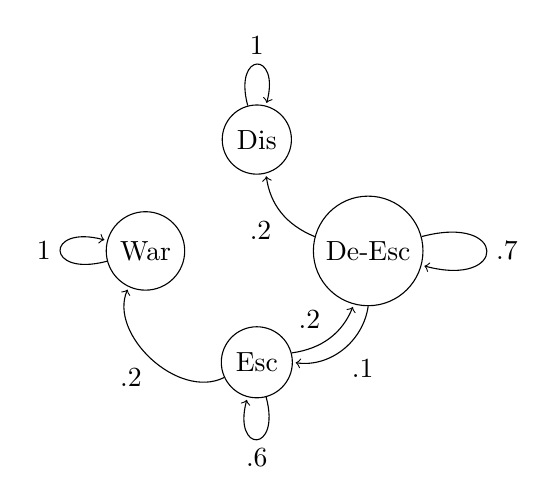
\begin{tikzpicture}[shorten >=1pt,node distance=2cm,on grid,auto]
   \node[state] (q_0) {War};
   \node[state] (q_1) [above right=of q_0] {Dis};
   \node[state] (q_2) [below right=of q_0] {Esc};
   \node[state] (q_3) [below right=of q_1] {De-Esc};
   \path[->]
    (q_0)   edge [loop left] node {1} ()
    (q_1)   edge [loop above] node {1} ()
    (q_2)   edge [bend left=70] node {.2} (q_0)
            edge [loop below] node {.6} ()
            edge [bend right] node {.2} (q_3)
    (q_3)   edge [bend left] node {.2} (q_1)
            edge [bend right=-45] node {.1} (q_2)
            edge [loop right] node {.7} ();
\end{tikzpicture}
\end{center}
% \end{minipage}

\item The National League and American League used to alternate as hosts for the opening game of
each year’s World Series. Show that this process can be set up as a Markov process with transition
matrix
\[
P=
\left(
\begin{array}{c c}
0 & 1\\
1 & 0
\end{array}
\right)
\]
\begin{quote}
Since the venues are alternating, there is a 100\% chance that the venue will change, and a 0\%
chance it will stay the same.
\end{quote}

\item A particle moves along a line from an initial position 2 feet to the right of the origin.
Each minute it moves one foot to the right with probability 1/2 or 1 foot to the left. There
are barriers at the origin and 4 feet to the right of the origin; if the particle hits a barrier,
it remains there. Show that this process can be set up as a Markov process with five states.
Determine the transition matrix and draw the state diagram.

\begin{minipage}{0.5\textwidth}
\[
\begin{array}{c | c c c c c}
& \text{L} & \text{R} & \text{S} & \text{RB} & \text{LB}\\
\hline
\text{L} & .25 & .5 & 0 & 0 & .25\\
\text{R} & .5 & .25 & 0 & .25 & 0\\
\text{S} & 0 & 0 & 1 & 0 & 0\\
\text{RB} & 0 & 0 & 1 & 0 & 0\\
\text{LB} & 0 & 0 & 1 & 0 & 0
\end{array}
\]
\end{minipage}
\begin{minipage}{0.5\textwidth}
\begin{center}
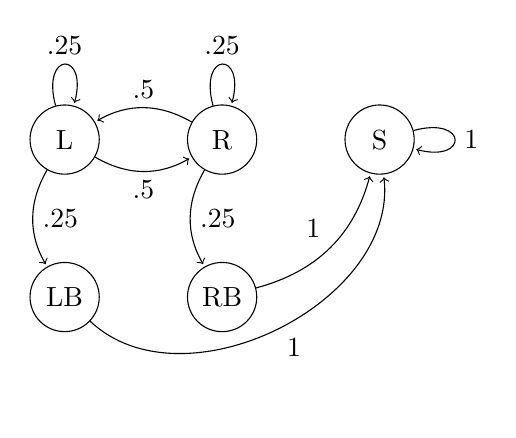
\begin{tikzpicture}[shorten >=1pt,node distance=2cm,on grid,auto]
   \node[state] (left) {L};
   \node[state] (right) [right=of left] {R};
   \node[state] (rb) [below=of right] {RB};
   \node[state] (lb) [below=of left] {LB};
   \node[state] (stop) [right=of right] {S};
   \path[->]
        (left)  edge [loop above] node {.25} ()
                edge [bend right, swap] node {.5} (right)
                edge [bend right] node {.25} (lb)
        (right) edge [loop above] node {.25} ()
                edge [bend right] node {.25} (rb)
                edge [bend right, swap] node {.5} (left)
        (stop)  edge [loop right] node {1} ()
        (lb)    edge [bend right=70, swap] node {1} (stop)
        (rb)    edge [bend right] node {1} (stop);
\end{tikzpicture}
\end{center}
\end{minipage}

\item The random walk of Exercise 6 is modified so that if the particle reaches the barrier at the
origin, it must move one foot to the right in the next minute, while if it hits the other barrier,
it must move one foot to the left in the next minute. Determine the transition matrix for the
associated Markov chain.
\[
\begin{array}{c | c c c c c}
& \text{L} & \text{R} & \text{S} & \text{RB} & \text{LB}\\
\hline
\text{L} & .25 & .5 & 0 & 0 & .25\\
\text{R} & .5 & .25 & 0 & .25 & 0\\
\text{S} & 0 & 0 & 1 & 0 & 0\\
\text{RB} & 1 & 0 & 0 & 0 & 0\\
\text{LB} & 0 & 1 & 0 & 0 & 0
\end{array}
\]

\item Find the probability that a woman whose birthweight was average has a granddaughter with an
average birthweight.
\[
\begin{array}{c | c c}
& \text{Average} & \text{Not Average}\\
\hline
\text{Average} & .5 & .5\\
\text{Not Average} & .5 & .5
\end{array}
\]
\begin{quote}
The probability that a granddaughter will have average weight is $(.5)(.5)=.25$.
\end{quote}

\item Sketch the state diagram for the Lower Pine Cone College example.
\begin{center}
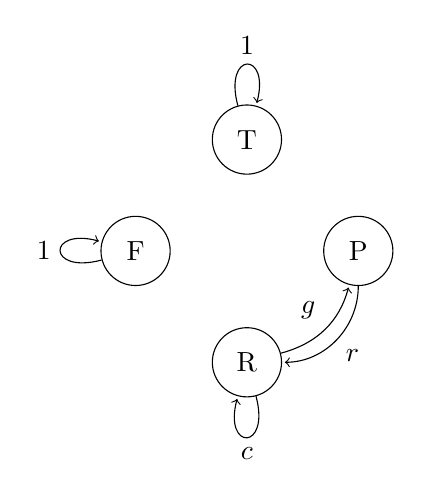
\begin{tikzpicture}[shorten >=1pt,node distance=2cm,on grid,auto]
   \node[state] (q_0) {F};
   \node[state] (q_1) [above right=of q_0] {T};
   \node[state] (q_2) [below right=of q_0] {R};
   \node[state] (q_3) [below right=of q_1] {P};
   \path[->]
    (q_0)   edge [loop left] node {1} ()
    (q_1)   edge [loop above] node {1} ()
    (q_2)   edge [loop below] node {$c$} ()
            edge [bend right] node {$g$} (q_3)
    (q_3)   edge [bend right=-45] node {$r$} (q_2);
\end{tikzpicture}
\end{center}

\setcounter{enumi}{10}

\item Using probabilistic considerations only, show that the square of a stochastic matrix is also a
stochastic matrix.
\begin{quote}
If it was not a stochastic matrix, then there would be no way to represent the next state in the
system. The total probability of all the transitions must sum to 1, since there is a 100\% chance
of a transition occurring in every step of the chain.
\end{quote}

\item A stochastic matrix is doubly stochastic if the sum of the entries in each column is 1. If $A$
and $B$ are doubly stochastic square matrices, is $A^{2}$ doubly stochastic? Is $AB$?
\begin{quote}
Yes, the square of a doubly stochastic matrix is still a doubly stochastic matrix. $AB$ is also
still doubly stochastic.
\end{quote}

\item Write out inductive proofs for Theorems 2 and 3.

\item Use matrix multiplication to solve Exercise 8.
\[
\left(
\begin{array}{c c}
.5 & .5\\
.5 & .5
\end{array}
\right)
\cdot
\left(
\begin{array}{c c}
.5 & .5\\
.5 & .5
\end{array}
\right)
=
\]

\item Abigail bought a toy with her allowance this week (see Exercise 2). Find the probability that
she will buy a toy 4 weeks from now.

\item Find the distribution of birth weights (Example 1) after one generation if the initial
probability distribution is (.4, .3, .3).

\item Suppose the distribution of birth weights of a generation of daughters is
$p^{(1)}=7(0.31,0.45,0.24)$. Can you find the distribution of birth weights of the mothers?

\item Use the state diagram in Fig. 11.3 to find the probability that the process reaches state
$S_{3}$ in two steps if it starts in state $S_{1}$.

\item Let $P$ be the transition matrix of Eq. (4). Compute $P^{2}$. What can you say about the
first column of $P^{3}$ and $P^{n}$?

\setcounter{enumi}{20}
\item The matrices determined in Exercises 1-7 are all transition matrices for Markov processes.
Which ones are regular?
\begin{quote}
Exercises 1 and 2 are regular matrices, since they have all positive entries.
\end{quote}

\item Find, if possible, a fixed-point vector for each of the transition matrices of Exercises 1-7.
\begin{multicols}{2}
\begin{enumerate}
\item $\displaystyle \mathbf{w}=\left\{{5\over9}, {4\over9}\right\}$
\item $\displaystyle \mathbf{w}=\left\{{4\over7}, {3\over7}\right\}$
\item $\displaystyle \mathbf{w}=\left\{{23\over70}, {43\over70}, {2\over35}\right\}$
\item This is not a regular matrix, so no $\bf{w}$ exists.
\item This is not a regular matrix, so no $\bf{w}$ exists.
\item This is not a regular matrix, so no $\bf{w}$ exists.
\item This is not a regular matrix, so no $\bf{w}$ exists.
\end{enumerate}
\end{multicols}

\item Does a matrix of the form
$\displaystyle A=\left(\begin{array}{c c}a & b \\ -b & d\end{array}\right)$ have a fixed-point vector?
\begin{quote}
If it has a fixed-point vector, then that vector is given by
\[
\mathbf{w}=\left\{ {c\over b+c},{b\over b+c} \right\}
= \left\{ {-b\over b-b},{b\over b-b}\right\}
= \left\{ {-b\over 0},{b\over 0}\right\}.
\]
Therefore, there is no fixed-point vector for the matrix.
\end{quote}

\setcounter{enumi}{31}
\item Which of the transition matrices of Exercises 1-7 represent absorbing Markov processes?
\begin{quote}
Exercises 4 and 6 represent absorbing Markov processes, since they have nodes which are not
escapable.
\end{quote}
\end{enumerate}

\end{document}
